\subsection{Task 2.2 -- Sequence diagram}
% SVG: java -DPLANTUML_LIMIT_SIZE=16384 -jar plantuml.jar -charset UTF-8 -tsvg docs/diagrams/sequence-checkout.puml
% PNG: java -DPLANTUML_LIMIT_SIZE=16384 -jar plantuml.jar -charset UTF-8 -Sdpi=200 -tpng docs/diagrams/sequence-checkout.puml

\textbf{Sequence-01} mô tả chi tiết tương tác tuần tự giữa các thành phần trong use-case \textbf{UC-CK: Đặt và thanh toán đơn hàng} (Task~1.3), bám sát các yêu cầu chức năng (FR-05, FR-06, FR-07, FR-08, FR-10, FR-13) và phi chức năng (NFR-01, NFR-02) đã đặc tả trong SRS Task~1.2.
Hình~\ref{fig:sequence-checkout} mô hình hóa toàn bộ vòng đời của một đơn hàng từ trang giỏ hàng đến khi hoàn tất thanh toán hoặc hủy đơn.

Sơ đồ bao gồm 6 lifeline:
\begin{enumerate}
  \item \textbf{Khách hàng (CUSTOMER)}: Actor thực hiện thao tác đặt hàng, chọn phương thức thanh toán và chuyển tiền.
  \item \textbf{Next.js UI (Giao diện)}: Client-side web application xử lý hiển thị, lưu giỏ hàng trong \texttt{localStorage}, xác thực sơ bộ và thực hiện polling trạng thái.
  \item \textbf{NestJS API (Backend)}: Hệ thống máy chủ ứng dụng đảm nhận xác thực JWT, kiểm tra DTO, điều phối nghiệp vụ và bảo vệ dữ liệu bằng transaction.
  \item \textbf{PostgreSQL (Cơ sở dữ liệu)}: Lưu trữ dữ liệu quan hệ, đảm bảo tính toàn vẹn (ACID), hỗ trợ khóa lạc quan (\emph{optimistic locking}) cho nguyên liệu và khóa bi quan (\emph{pessimistic locking}) cho thanh toán.
  \item \textbf{Ngân hàng giả lập (Mock Bank)}: Cổng thanh toán giả lập tiếp nhận thao tác chuyển tiền QR và phản hồi trạng thái.
  \item \textbf{Nhân viên (ADMIN)}: Quản trị viên/thu ngân đối chiếu sao kê thực tế và ra quyết định xác nhận hoặc từ chối thanh toán.
\end{enumerate}

\subsubsection{Các giai đoạn và cơ chế xử lý}

Quy trình tuần tự được phân chia thành 4 giai đoạn rõ ràng:

\paragraph{Giai đoạn 1: Đặt đơn hàng (\texttt{POST /orders})}
Khách hàng bấm \emph{Đặt hàng} từ trang giỏ hàng (\texttt{/cart}). Next.js UI kiểm tra token JWT; nếu chưa đăng nhập, khách được chuyển hướng sang trang đăng nhập (\texttt{/login?redirect=/cart}) mà vẫn bảo toàn nguyên vẹn giỏ hàng trong \texttt{localStorage}.
Khi gửi yêu cầu \texttt{POST /orders}, client đính kèm JWT và \texttt{Idempotency-Key} trên HTTP header.
Backend thực hiện:
\begin{itemize}
  \item Kiểm tra hợp lệ DTO và JWT (lỗi trả về HTTP 400 hoặc 401).
  \item Mở transaction cơ sở dữ liệu: kiểm tra chống trùng lặp qua bảng khóa yêu cầu đơn hàng \texttt{order\_request\_keys}. Nếu cùng key và cùng dữ liệu món thì trả lại đơn hàng cũ (không tạo trùng); nếu cùng key nhưng khác dữ liệu món thì từ chối với HTTP 409 Conflict.
  \item Truy vấn giá gốc từ bảng \texttt{products} kết hợp phụ phí size/topping để tính lại giá (tuyệt đối không tin cậy giá gửi từ client do không có bảng \texttt{toppings} riêng biệt).
  \item Kiểm tra định lượng công thức và tồn kho nguyên liệu trong kho bằng \emph{optimistic locking}. Nếu không đủ nguyên liệu, transaction được rollback toàn bộ, trả về HTTP 400 và giữ nguyên giỏ hàng của khách (E1).
  \item Trừ tạm thời số lượng nguyên liệu trong kho để giữ chỗ; kiểm tra và giữ một lượt sử dụng voucher (nếu có).
  \item Tạo đơn hàng ở trạng thái \texttt{PENDING} với thời hạn thanh toán được gán vào trường \texttt{expiresAt = NOW() + 15m}, lưu \texttt{order\_items} và ghi nhận bản ghi vào \texttt{order\_request\_keys}. Trả về HTTP 201 Created kèm tổng tiền \texttt{total}.
\end{itemize}

\paragraph{Giai đoạn 2: Khởi tạo thanh toán \& Quét QR (\texttt{POST /payments})}
Khách hàng chọn phương thức \emph{Chuyển khoản / Ví} (\texttt{WALLET}) trên trang \texttt{/checkout/:orderId}. Giao diện gửi yêu cầu \texttt{POST /payments}. Backend xác thực đơn hàng thuộc quyền sở hữu của khách, đang ở trạng thái \texttt{PENDING} và còn hiệu lực trong 15 phút. Hệ thống ghi nhận khóa yêu cầu thanh toán vào bảng \texttt{payment\_request\_keys} và tạo bản ghi phiên thanh toán ở trạng thái \texttt{PENDING} với số tiền lấy từ đơn hàng, sinh đường dẫn QR và chuyển hướng khách sang màn hình thanh toán \texttt{/pay/:paymentId}.
Nếu client gửi lại cùng \texttt{Idempotency-Key} (ví dụ do mạng chậm hoặc bấm đúp) cho cùng đơn và cùng phương thức, backend trả lại phiên thanh toán cũ, không tạo phiên mới; nếu key đã dùng cho đơn hoặc phương thức khác thì trả HTTP 400.

\paragraph{Giai đoạn 3: Chuyển tiền qua Ngân hàng giả lập \& Kiểm tra thời hạn 15 phút}
Khách hàng quét mã QR để mở trang ngân hàng giả lập (\texttt{/mock-bank/:paymentId}, trang mở không yêu cầu đăng nhập) và bấm \emph{Chuyển tiền}. Ngân hàng giả lập gọi \texttt{POST /mock-bank/payments/:id/transfer} sang API. Tùy theo thời điểm thực tế, hệ thống rẽ nhánh xử lý:
\begin{itemize}
  \item \textbf{[Khách chuyển tiền trước hạn -- \texttt{expiresAt > NOW()}]:}
    Trong một transaction, API ghi nhận giao dịch tiền vào (\texttt{IN}) trên bảng \texttt{bank\_transactions} và cập nhật trạng thái phiên thanh toán thành \texttt{TRANSFER\_RECEIVED}. 
    \textbf{Đặc biệt quan trọng:} Đơn hàng \textbf{vẫn giữ nguyên trạng thái \texttt{PENDING}}, không tự động chuyển thành \texttt{PAID} để chống tác vụ nền tự hủy quá hạn vì tiền thực tế đã về tài khoản, đồng thời tuân thủ nguyên tắc chỉ có nhân viên mới được quyền xác nhận đơn.
  \item \textbf{[Hết 15 phút chưa chuyển / Quá hạn -- \texttt{expiresAt < NOW()}]:}
    Tác vụ nền (\emph{Background Job}) hoặc API tự động kiểm tra, nếu đơn vẫn ở trạng thái \texttt{PENDING} và chưa nhận được khoản chuyển khoản nào (\texttt{TRANSFER\_RECEIVED}), hệ thống mở transaction cập nhật trạng thái đơn thành \texttt{CANCELLED}, hoàn trả lại nguyên liệu vào kho đúng một lần và khôi phục lại lượt dùng voucher cho khách.
\end{itemize}

\paragraph{Giai đoạn 4: Đối chiếu sao kê, Polling và Xử lý kết quả}
Trên giao diện Admin (\texttt{/admin/payments}), nhân viên nhận thông báo và danh sách giao dịch mới thông qua polling định kỳ mỗi 4 giây. Song song đó, giao diện khách hàng tại trang \texttt{/pay/:paymentId} thực hiện polling mỗi 3 giây (\texttt{GET /payments/:id}) để cập nhật trạng thái. Nhân viên đối chiếu số tiền và nội dung chuyển khoản với sao kê thực tế:
\begin{itemize}
  \item \textbf{Trường hợp 1 -- Nhân viên xác nhận thanh toán (Thành công):}
    Nhân viên bấm \emph{Xác nhận} (\texttt{POST /admin/payments/:id/confirm}). Backend sử dụng khóa bi quan (\emph{pessimistic locking}) trên dòng phiên và dòng đơn hàng, cập nhật phiên sang \texttt{SUCCESS}, chuyển đơn hàng từ \texttt{PENDING} $\rightarrow$ \texttt{PAID} (thông qua hàm kiểm tra ràng buộc chuyển trạng thái \texttt{assertTransition}), cập nhật trạng thái sử dụng voucher thành \texttt{VoucherUsage.status = USED} và tích lũy điểm thưởng (+1 điểm cho mỗi 10.000~VNĐ thực trả).
    Khi client của khách hàng nhận kết quả \texttt{PAID} qua polling, giỏ hàng trong \texttt{localStorage} mới chính thức được xóa bỏ và giao diện tự động chuyển hướng sang màn hình xác nhận đơn (\texttt{/orders/:id/confirmation}).
  \item \textbf{Trường hợp 2 -- Nhân viên từ chối thanh toán (Thất bại / Thử lại):}
    Nếu thông tin chuyển khoản không khớp, nhân viên bấm \emph{Từ chối} (\texttt{POST /admin/payments/:id/reject}). Backend cập nhật phiên thành \texttt{FAILED}, chuyển đơn hàng sang \texttt{PAYMENT\_FAILED}, đồng thời tự động ghi nhận một giao dịch hoàn tiền (\texttt{REFUND}) trên bảng \texttt{bank\_transactions} đúng bằng số tiền đã nhận.
    Nguyên liệu đã giữ và giỏ hàng của khách \textbf{vẫn được bảo lưu}. Khách hàng được thông báo thất bại và có thể bấm nút \emph{Thử lại thanh toán} ngay trên cùng mã đơn hàng với khóa yêu cầu thanh toán mới. Khi đó đơn chuyển từ \texttt{PAYMENT\_FAILED} về \texttt{PENDING} và tạo phiên thanh toán mới (thời hạn 15 phút vẫn tính từ lúc tạo đơn ban đầu, không được gia hạn).
\end{itemize}

\begin{figure}[p]
  \centering
  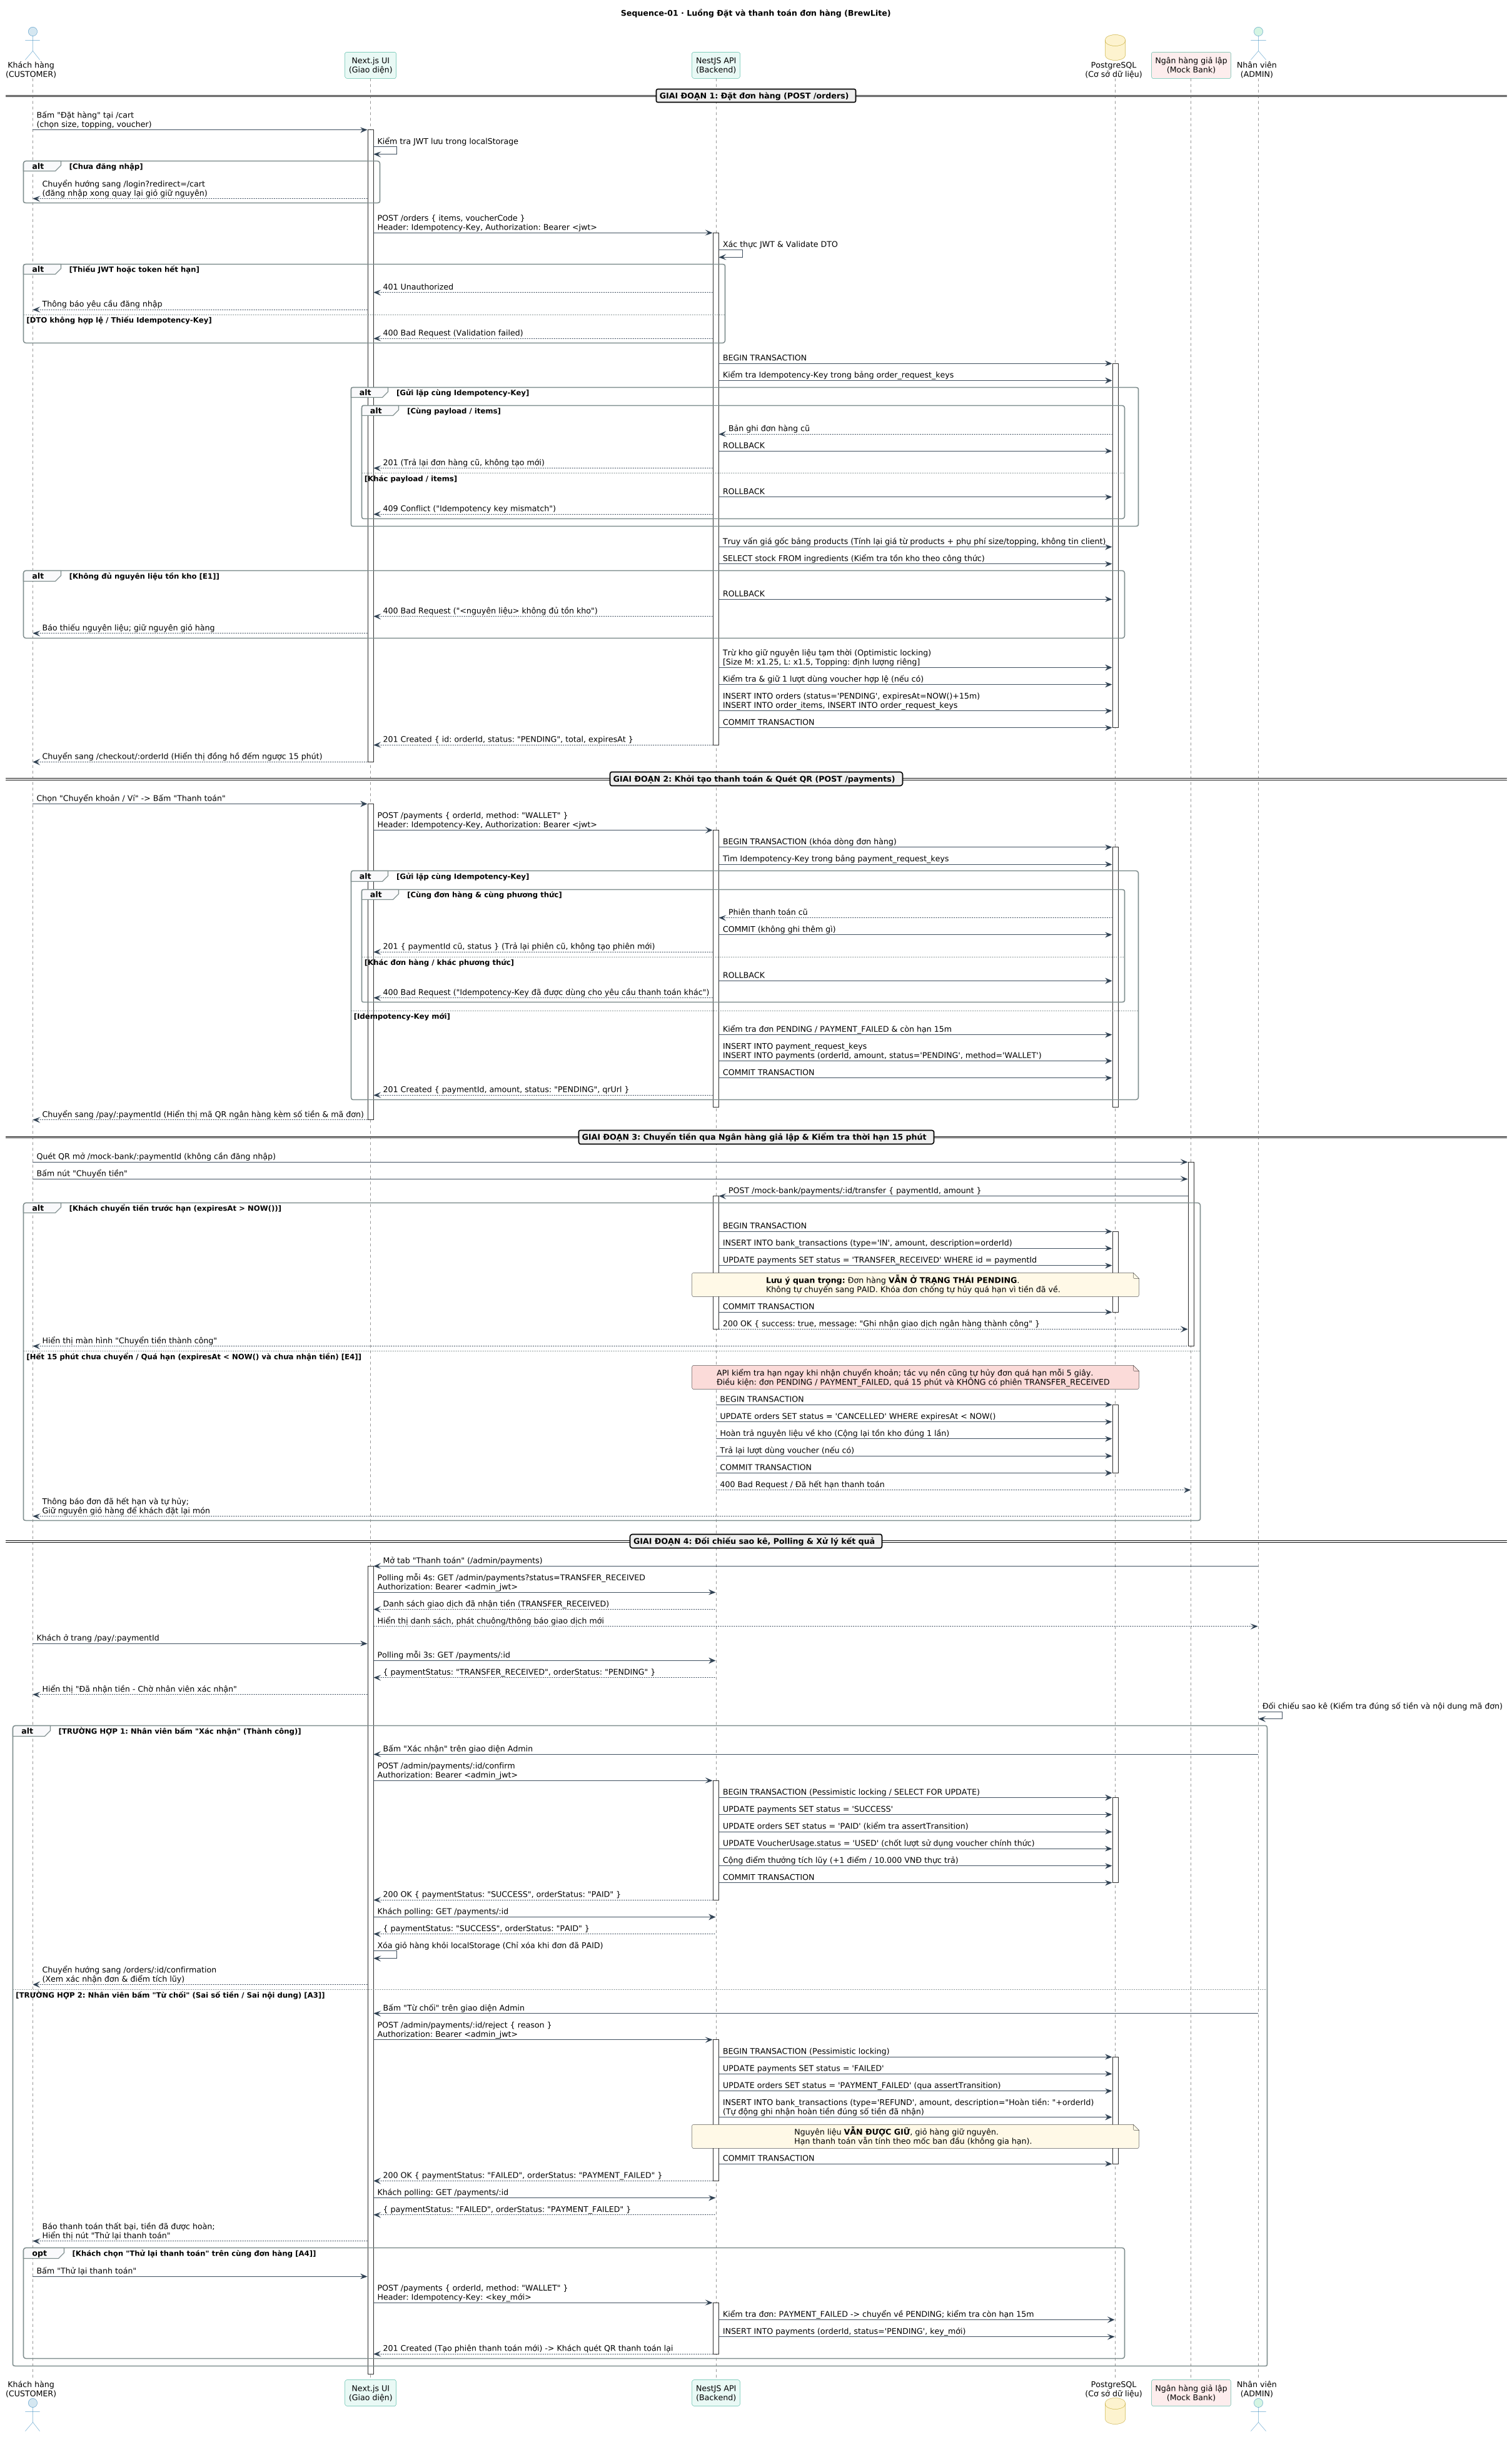
\includegraphics[width=\textwidth,height=0.93\textheight,keepaspectratio]{docs/diagrams/sequence-checkout.png}
  \caption{Sequence-01: Sơ đồ tuần tự Đặt và thanh toán đơn hàng (BrewLite).}
  \label{fig:sequence-checkout}
\end{figure}

\subsubsection{Truy vết yêu cầu}

Sơ đồ \textbf{Sequence-01} bao phủ đầy đủ và hiện thực hóa các yêu cầu kỹ thuật:
\begin{itemize}
  \item \textbf{FR-03, FR-04}: Bảo toàn giỏ hàng qua \texttt{localStorage}; bảo vệ API bằng JWT và phân quyền \texttt{ADMIN}.
  \item \textbf{FR-05, FR-06}: Đặt đơn hàng kèm giữ chỗ nguyên liệu theo công thức bằng \emph{optimistic locking}; hoàn kho tự động khi hết hạn.
  \item \textbf{FR-07, FR-08}: Tích hợp ngân hàng giả lập qua mã QR, ghi nhận giao dịch vào bảng \texttt{bank\_transactions}, nhân viên đối chiếu và xác nhận thanh toán (\emph{pessimistic locking}), tự động tạo giao dịch hoàn tiền \texttt{REFUND}.
  \item \textbf{FR-10}: Máy trạng thái đơn hàng nghiêm ngặt (\texttt{assertTransition}): \texttt{PENDING} $\rightarrow$ \texttt{PAID}, \texttt{PENDING} $\rightarrow$ \texttt{PAYMENT\_FAILED} $\rightarrow$ \texttt{PENDING}, và tự hủy \texttt{CANCELLED} sau 15 phút.
  \item \textbf{FR-13}: Tích hợp mã giảm giá và cộng điểm thưởng khi đơn hoàn tất.
  \item \textbf{NFR-01, NFR-02}: Chống tạo trùng lặp giao dịch thông qua các bảng khóa yêu cầu \texttt{order\_request\_keys} và \texttt{payment\_request\_keys}; kiểm soát truy cập đồng thời và an toàn dữ liệu tài chính.
\end{itemize}
Cột \emph{Thiết kế / Sơ đồ} trong ma trận truy vết (\texttt{docs/traceability-matrix.md}) được cập nhật tương ứng với nhãn \textbf{Sequence-01}.
